\chapter{Preliminaries}

\section{Submanifolds}

Often in mathematics there is an obvious notion of a ``subobject'': given a structure on a set there is a simple way to restrict it to a subset, such that the subset can be said to have the same structure.
For example, the structure on a group is the identity element, inversion, and multiplication; if there is a subset containing the identity element and which is preserved under inversion and multiplication, then we have a subgroup.
Or for a topological space $X$, any subset $A$ has a topology given by intersection of open sets of $X$ with $A$.
The structures on the subset can often be characterized by the fact that they make the inclusion map $A \hookrightarrow X$ a structure preserving map (group homomorphism and continuous map respectively for the two examples).

In the case of manifolds however the definition of a submanifold is not as trivial and there are several notions that have strong claims for the title.
To complicate matters, the notion that is the most widely taught (embedded submanifolds) is not the one that is most appropriate for Lie group theory.
Let us begin by summarizing the common definitions.

\begin{definition}\textup{\cite[Def~1.27, Rem~1.33]{Warner1983},\cite[Defs~1.1.36,~1.1.40,~1.2.10,~1.2.21]{Sharpe1997}} \\
Let $\phi : N \to M$ be a smooth map of manifolds.
\begin{enumerate}
\item 
$\phi$ is called an \emph{immersion} if $d\phi_p : T_pN \to T_{\phi(p)}M$ is injective at every point $p \in N$.
The pair $(N,\phi)$ is called an \emph{immersed manifold} in $M$.
% \item 
% $\phi$ is called a submersion if $d\phi_p : T_pN \to T_{\phi(p)}M$ is surjective at every point $p \in N$.
\item
If $\phi$ is an injective immersion then the pair is called an \emph{immersed submanifold}.
\item 
Two immersed submanifolds $(N_1,\phi_1)$ and $(N_2,\phi_2)$ are called \emph{equivalent} if there is a diffeomorphism $\varphi : N_1 \to N_2$ such that $\phi_1 = \phi_2 \circ \varphi$.
\item
If an injective immersion $\phi$ has the property that for every smooth map $f: S \to M$ with $f[S] \subset \phi[N]$ the map $\phi^{-1} \circ f : S \to N$ is smooth, then we call $\phi$ a \emph{weak embedding} and the pair a \emph{weakly embedded submanifold}.
\item
If an immersion $\phi$ is a homeomorphism from $N$ to $\phi(N)$, the latter with the subspace topology of $M$, then we call it an \emph{embedding} and the pair is called an \emph{embedded submanifold}.
\item
A continuous function between Hausdorff spaces is called \emph{proper} if the preimage of a compact set is always a compact set.
A proper immersion submanifold is called a \emph{proper submanifold}.
\item
When we say \emph{submanifold}, we generally mean a weakly embedded submanifold.
\end{enumerate}
\end{definition}

This is a lot of terminology, but it harmonizes the definitions in Sharpe and Warner, see below table.
It is in fact a strict hierarchy: each type of submanifold is a subtype of the previous.

\begin{table}[ht]
\begin{tabular}{l|l|l}
 & Sharpe & Warner \\ \hline
immersed manifold & immersed manifold & \\
immersed submanifold & immersed submanifold & submanifold \\
weakly embedded submanifold &  &  \\
 & submanifold &  \\
embedded submanifold & regular submanifold & imbedding \\
proper submanifold & proper submanifold & proper submanifold \\
\end{tabular}
\end{table}

To return to the discussion of the first paragraph, restriction vs inclusion, these definitions are given in terms of a smooth map into $M$, which is to say the perspective of inclusion.
So the question from the perspective of restriction is whether the manifold structure of $N$ is determined or can be recovered solely from the image $\phi[N]$.
There is a simple example that shows that not even the topology of $N$ is determined for an immersed submanifold: consider the subset $\{x^2 = y^2\} \subset \bbR^2$.
We can split this into a line and two rays in two ways.
Therefore immersed submanifolds must always be given with the immersion $\phi$.

On the other hand, by using the implicit function theorem the preimage of a regular value is an embedded submanifold.
The idea is to take the construction of charts in the implicit function theorem and generalize it to weakly embedded submanifolds.

\begin{definition}
\label{def:plaques}
\textup{\cite[Def~1.2.1,1.2.2,Thm~1.2.7]{Sharpe1997}} \\
Any subset $A$ let $C(A,x)$ be points that can be reached from $x$ by a continuous path through $A$.
Let $N' \subset M$ be a subset.
Given a chart $\varphi: U \subset M \to \bbR^m$ we say that $W = C(N'\cap U,x)$ is a \emph{flat plaque} if 
\[
\varphi(W) = \varphi[U] \cap (\bbR^n \times 0) \subset \bbR^n \times \bbR^{m-n},
\]
an open subset of an $n$-dimensional affine subspace of $\bbR^m$.
In that case $\varphi|_W$ is called a plaque chart of $W$.
The \emph{submanifold topology} on $N'$ is the topology such that flat plaques are open.
In general the submanifold topology is finer (has more open sets) than the subspace topology~\cite[Def~1.2.4]{Sharpe1997}.
\end{definition}

\begin{figure}[ht]
\begin{center}
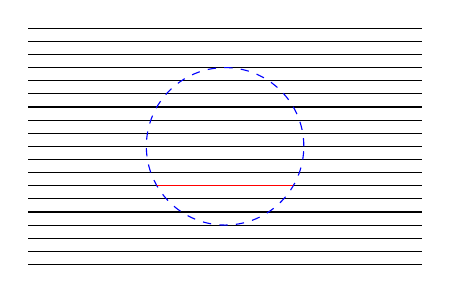
\begin{tikzpicture}[scale=0.5]
  % Draw 10 vertical lines closely bunched together
  \foreach \x in {0,1,2,...,18} {
    \draw (0,\x/3) -- (10,\x/3);
  }
  
  % Draw the circle
  \draw[dashed,blue] (5,3) circle (2);
  
  % Highlight one of the line segments in the circle
  \draw[red] (5-1.73,2) -- (5+1.73,2);
\end{tikzpicture}
\caption{$N'$ is the collection of black lines. The interior of the blue disc is an open subset of the plane $U$, and the red segment is a plaque.}
\end{center}
\end{figure}

Some commentary before we slot this into our hierarchy.
The definition of submanifold in~\cite{Sharpe1997} requires a collection of charts $(U_\alpha, \varphi_\alpha)$ of $M$ covering $\overline{N'}$ such that the connected components of $U_\alpha \cap N'$ are all flat plaques.
This has the effect of excluding the following example.
Consider $N$ as a countable collection of spheres and take $\phi : N \to \bbR^3$ to be the map that embeds the $k$th sphere as $\partial B(k^{-1}, 0.5(k+1)^{-2})$; one has a sequence of non-overlapping spheres decreasing in size with the origin as a limit point.
In particular any neighborhood $U$ of the origin must contain a sphere as a connected component of $U \cap N' = \phi[N]$, but a sphere cannot be a flat plaque.
Sharpe calls this an `odd limit point', but it seems no more odd than a collection of lines immersed as $\{n^{-1}\} \times \bbR \subset \bbR^2$, which is allowed by the definition.
If one truly wishes to avoid odd limits, an embedded submanifold is the correct notion.
Instead, it would be better to say that Sharpe is concerned with foliations, and this shrinking chain of spheres cannot be part of a regular foliation.
For embedded submanifolds the subspace and submanifold topologies coincide~\cite[Prop~1.2.9]{Sharpe1997}.
The example of the dense wrapping of the line around a torus is the classic example of a submanifold in Sharpe's sense that is not embedded.

It is also important that we use paracompact manifolds, which is equivalent to each connected component being second countable.
This is because a subset of $M$ need not be second countable in the submanifold topology.
Consider the example of the irrational numbers in the real line.
The flat plaques are the sets $\{x\}$ for any irrational $x$.
Thus the submanifold topology is the discrete topology, which is not second-countable.

\begin{theorem}
\label{thm:weakly embedded submanifold}
\textup{\cite[Thm~1.2.7]{Sharpe1997}\cite[Lems~I.2.15--17]{Kolar1993}} \\
Let $N' \subset M$ be a subset.
Suppose for every point $x \in N'$ there is a chart making $C(N'\cap U,x)$ is a flat plaque of dimension $n$.
Let $N$ be the set $N'$ with the submanifold topology and a smooth atlas comprised of the plaque charts.
Then $N$ is a manifold and the inclusion map is a weak embedding.
Conversely, if $\phi : N \to M$ is a weak embedding then this reconstructs the atlas of $N$.
\end{theorem}
\begin{proof}
Because we have weakened the conditions, the proof in~\cite[Thm~1.2.7(i)]{Sharpe1997} no longer works.
I am not completely convinced by~\cite[Lems~I.2.15--17]{Kolar1993} because it uses a Riemannian metric, but the usual proof that a Riemannian metric induces the topology of a space already assumes that you have a topological manifold.
The arguments below attempt to add fill out the details on their idea.

A subspace of a Hausdorff space is Hausdorff, and the submanifold topology is finer than the subspace topology.
Hence $N$ is Hausdorff too.
We can argue in the same way for the other separation axioms, and that $N$ is locally compact.

To show that $N$ is paracompact, we need to show that each connected component $N_0 \subset N$ is second countable.
Necessarily $N_0$ is contained in a connected component $M_0 \subset M$, which is second countable since $M$ is paracompact.
We apply Urysohn's metrization theorem, which says that $M_0$ is metricizable, to get a distance function $d$.
Now $N_0$ is a metric space using the restriction of $d$, but this induces the subspace topology, not necessarily the submanifold topology.
Instead we use the intrinsic distance function $d'$, which is the infimum of path lengths in $N_0$ measured with $d$.

In general, $d' > d$, and we may worry that although $N_0$ is path connected, some paths might be infinitely long, and hence $N_0$ would not be a metric space.
To see that this is not the case, for any point $x \in N_0$ consider first a flat plaque $W \ni x$.
We use $\varphi$ to move everything to $\bbR^m$.
Shrinking the chart if necessary, we can assume that $U$ is convex.
$d$ induces a distance function on $\bbR^n \supset W$.
Therefore the intrinsic distance between any points of $W$ is finite, because the length of a chord is an upper bound.
A path between two points of $N_0$ is compact, and therefore covered by finitely many `convex' flat plaques.
The triangle equality now ensures that the path length is finite.

In fact for any open set $V$ of $N_0$, choose any point $x \in V$.
We consider the convex flat plaque centered at $x$ from the previous paragraph.
The set $V \cap W$ is an open subset of the affine subspace, so there is an open set $\tilde{V} \subset U \subset \bbR^n$ with $\tilde{V} \cap W = V \cap W$.
Because $d$ generates the topology of $U$, there is some ball $B_d(x,r) \subset \tilde{V}$.
By a standard argument, any path that leaves $B_d(x,r) \cap W$ has length at least $r$, so $B_{d'}(x,r) \subset B_d(x,r) \cap W$. 
Hence we have found an open ball with respect to $d'$ centered at $x$ contained in $V$.
As we can do this for every point of $V$, $d'$ induces the submanifold topology.

Lastly,~\href{https://math.stackexchange.com/questions/10885/non-separable-locally-compact-connected-metric-space}{MSE} tells us that a connected locally-compact metric space is second countable.
By definition, the plaque charts form a smooth atlas.
Therefore we have shown that $N_0$ is a manifold.

That this is a weak embedding is~\cite[Thm~1.2.7(iii)]{Kolar1993}.

The converse follows from~\cite[I.2.15~Lemma]{Kolar1993} (the construction can be carried out on the image of a weak embedding) and~\cite[Lemma~1.1.41]{Sharpe1997} (a weak embedding is compatible with a unique manifold structure).
\end{proof}

Finally, by \cite[Thm~1.2.11]{Sharpe1997} proper submanifolds are automatically embedded, so we have a strict hierarchy of conditions.
The standard example of an embedded submanifold that is not proper is $(0,1) \subset \bbR$.
We see that a sequence in $N$ may converge to a point of $M\setminus N$.

These constructions answer the question of how to endow a subset with a manifold structure.
There is the possibility however that there are different constructions.
Warner addresses these concerns with the following theorem: 
\begin{theorem}
\label{thm:submanifolds}
\textup{\cite[Remark~1.33]{Warner1983}}
\begin{enumerate}
\item Let $M$ be a manifold and $A$ a subset of $M$. Fix a topology on $A$. Then there is at most one manifold structure on $A$ such that $(A,\phi)$ is an immersed submanifold of $M$, where $\phi$ is the inclusion map.
\item Again let $A$ be a subset of $M$. If $A$ with the subspace topology has a manifold structure such that $(A,\phi)$ is an immersed submanifold of $M$, then it is the unique topology on $A$ such that there exists a manifold structure for which $(A,\phi)$ is an immersed submanifold of $M$.
\end{enumerate}
\end{theorem}

We generalize Part (b) slightly below.
This generalization is stronger than~\cite[Lem~2.1.41]{Sharpe1997}, because we only require the inclusions to be injective immersions, not weak embeddings.

\begin{theorem}
\label{thm:unique manifold structure}
Let $A$ be a subset of $M$. 
If $A$ with the submanifold topology has a manifold structure such that $(A,\phi)$ is an immersed submanifold of $M$, then it is the unique topology on $A$ such that there exists a manifold structure for which $(A,\phi)$ is an immersed submanifold of $M$.
\end{theorem}
\begin{proof}
First we address the relationship between the manifold structure on $A$ and the plaque charts.
For any function $A \hookrightarrow M$ that is an immersion at $p$ the constant rank theorem gives us a plaque chart of $A$ at $p$.
Applying this to the inclusion $\phi$ and at every point we get that $A$ is a weakly embedded submanifold.
By Part (a) of the previous theorem this is the unique manifold structure on $A$ with the submanifold topology (the manifold structure supposed in this theorem and the plaque charts belong to the same maximal atlas).

Now we move on to the statement in the theorem.
For clarity, let $B$ the manifold that has the same points as $A$ but a different topology and manifold structure, and let its inclusion be $\psi : B \hookrightarrow M$.
In terms of points, the composition $\phi^{-1} \circ \psi : B \to A$ is the identity map, so bijective.
We know that $(A,\phi)$ is a weak embedding.
Hence $\phi^{-1} \circ \psi$ is in fact a smooth map of manifolds.
It must also be an immersion: if there is a smooth path $\alpha$ in $B$ such that $\phi^{-1} \circ \psi \circ \alpha$ represents the zero vector then $\psi \circ \alpha$ represents the zero vector in $M$ by applying $\phi$ and so $\alpha$ represents the zero vector using that $\psi$ is an immersion. 
At the final step of the proof of Part (b) of the above theorem, Warner uses his Exercise~1.6 to conclude that a smooth bijective immersion is a diffeomorphism.
We do the same.
\end{proof}


\section{Lie Brackets and Distributions}

It is common in a course on manifolds to study vector fields and their integral curves.
The key local result is
\begin{theorem}[Picard-Lindelöff]
\textup{\cite[Theorem~2.1.1]{Sharpe1997}}\cite[Theorem~1.2.1]{Ivey2016} \\
Let $F : J \times U \subset \bbR\times\bbR^n \to \bbR^n$ be a smooth time-dependent vector field. 
Assume $0 \in J$. 
Consider $u : \bbR \to U$ the system of ODEs $u'(t) = F(t,u(t))$.
For any $c \in U$ there exists an $\varepsilon > 0$ such that there is a unique solution smooth solution on $(-\varepsilon,\varepsilon)$ with $u(0) = c$.
Moreover, for any $p \in U$ there is an open neighborhood $p \in V \subset U$, $\varepsilon > 0$ and smooth map $u : (-\varepsilon,\varepsilon) \times V \to U$ such that $u(\cdot,c)$ is the unique solution with initial condition $c$.
\end{theorem}

If one has a smooth vector field on a manifold, then we can ask for a curve $\gamma$ through $p = \gamma(0)$, called an integral curve, such that the tangent vectors of $\gamma$ are equal to the vector field.
In other words, the integral curve is a solution to the time-independent ODE $\gamma'(t) = X(\gamma(t))$.
This theorem provides for the existence of integral curves of the vector field in every coordinate chart, and uniqueness means that they can be patched together to give unique maximal integral curves through every point.

The set of integral curves of a vector field $X$ define a flow of the manifold: $\tilde{X}_t(p)$ is defined to be equal to the integral curve of $X$ through $p$ at time $t$ (ie $t \mapsto \tilde{X}_t(p)$ is the integral curve).
This is a smooth function defined on a subset of $\bbR \times M$ (treating the subscript as the first variable here), in particular containing some neighborhood $(-\varepsilon,\varepsilon) \times U$ of any point $(0,p)$.
Uniqueness of the integral curves means that this flow is reversible.
Moreover, if the vector field is nonzero at a point, there is a chart containing that point where the vector field is the first coordinate vector $\partial_1$ and the flow is translation.
In the other direction, the derivative of the flow with respect to $t$ at $t=0$ gives back the vector field $X$.

The flow provides a way to connect points of a manifold with neighboring points, and so can be used to define a derivative, called the Lie derivative.
For example, for a function $f$
\[
\mathcal{L}_X f
= \lim_{h \to 0} h^{-1} \left( f \circ \tilde{X}_h - f \right)
= \left.\frac{d}{dt}\right|_{t=0} f \circ \tilde{X}_t
\]
is, by the chain rule, equal to $\langle X, f\rangle$.
The Lie derivative of a vector field is likewise defined by
\[
\mathcal{L}_X Y
= \lim_{h \to 0} h^{-1} \left( d\tilde{X}_{-h}(Y \circ \tilde{X}_h) - Y \right)
= \left.\frac{d}{dt}\right|_{t=0} d\tilde{X}_{-t} \circ Y \circ \tilde{X}_t
\]
which is well-defined since $d\tilde{X}_{-h}$ takes $T_{\tilde{X}_h(p)}M$ to $T_pM$.
Most importantly, the Lie derivative of a vector field is a type of commutator.
This is easiest to calculate in local coordinates, specifically the ones adapted to the flow of $X$~\cite[Thm~9.38]{Lee2012}.
If $Y(p) = Y^i(p) \partial_i|_p$ then
\begin{align*}
d\tilde{X}_{-h}(Y \circ \tilde{X}_h) (p)
&= d\tilde{X}_{-h} \left( Y^i(p + (h,0,\ldots)) \partial_i|_{\tilde{X}_h(p)} \right)
= Y^i(p + (h,0,\ldots)) \partial_i|_{p} \\
\mathcal{L}_X Y (p)
&= \lim_{h \to 0} h^{-1} \left( Y^i(p + (h,0,\ldots)) - Y^i(p) \right) \partial_i|_{p}
= \frac{\partial Y^i}{\partial x_1} \partial_i|_{p}.
\end{align*}
On the other hand, this is the commutator of $X$ and $Y$
\begin{align*}
[X,Y]
= \frac{\partial Y^i}{\partial x_1} \partial_i - Y^i\frac{\partial 1}{\partial x_i} \partial_1
= \frac{\partial Y^i}{\partial x_1} \partial_i.
\end{align*}
One can check that the commutator of two vector fields is a well-defined vector field, independent of the coordinates.
Therefore $\mathcal{L}_X Y = [X,Y]$.

From this commutator formula, most of the properties of the Lie derivative of vector fields easily follow.
For us, the most important are anti-symmetry $[X,Y] = -[Y,X]$ and the Jacobi identity $[X,[Y,Z]] = [[X,Y],Z] + [Y, [X,Z]]$.
There is also a generalization of adapted coordinates to sets of linearly-independent commuting vector fields: around each point there is a chart whose coordinates vector fields are the given vector fields.

We will need a generalization that deals with vector fields that are not commuting.
To motivate why this is geometrically interesting and not just generalization for its own sake, consider a submanifold $N$ inside $M$.
At each point $p \in N$ we can consider the vector subspace $T_pN \subset T_pM$.
At least locally, we can describe these subspaces as the span of independent vector fields.
The natural question is the converse: given a set of independent vector fields on $M$, does there exist a submanifold $N$ whose tangent space is their span?
For a single vector field, the answer is affirmative, namely the integral curve.

\begin{definition}
\textup{\cite[2.2.1,.2.2.2,2.3.2]{Sharpe1997}} \\
An $r$-dimensional distribution $\mathcal{D}$ on $M$ is a choice of an $r$-dimensional subspace $\mathcal{D}_p$ of $T_p M$ at every point $p \in M$.
It is called smooth if every point has a neighborhood and smooth vector fields $\{X_1, \dots, X_r \}$ that span the subspaces.
This is called a local basis for $\mathcal{D}$.
Equivalently, an $r$-dimensional distribution is a rank $r$ subbundle of $TM$.

A set of vector fields is called algebraically involutive if their Lie brackets are contained in their span.
Given two sets of vector fields with the same span, one is algebraically involutive if and only if the other is.
Therefore algebraically involutive is a property that is defined for distributions.

A distribution is called integrable if every point has a coordinate neighborhood in which the distribution is spanned by coordinate vector fields.
\\
A connected $r$-dimensional immersed submanifold $N$ is called an integral submanifold of $\mathcal{D}$ if at every point $T_pN = \mathcal{D}_p$.
\end{definition}

Consider the example of nested spheres centered at the origin in $\bbR^3\setminus\{0\}$. 
Their tangent planes define a $2$-distribution.
In a neighborhood of any point, suitable polar coordinates show that it is smooth and integrable.
However there don't exist global vector fields spanning this distribution, due to the hairy ball theorem (every vector field on a sphere vanishes at least once).
By definition, any of the spheres is an integral manifold of this distribution.

The important example of a non-integrable distribution is given in $\bbR^3$ by the planes normal to the vector field $n(x,y,z)=(y,-x,1)$~\cite[Ex~2.3.1]{Sharpe1997}.
There can be no integral manifold containing the origin.
Suppose there were.
Because the tangent plane at the origin is the $xy$-plane, we know that there is a neighborhood where is a graph over $x$ and $y$.
Now take a small loop in the integral manifold around the origin lying in this neighborhood.
Its height is monotonic, it doesn't close up.
This is a contradiction.
A local basis at the origin is given by $X_1 = \partial_x - y \partial_z$, $X_2 = \partial_y + x\partial z$.
Observe that $[X_1,X_2] = 2\partial_z$, so that it is not algebraically involutive.


If a distribution is integrable, then every point has an integral submanifold through it, just by taking a coordinate plane in an appropriate chart.
And if there is an integral submanifold of the distribution at a point, the local basis of the distribution gives a vector field on it.
So then the Lie bracket is again tangent to the integral submanifold, showing that the vector fields are algebraically involutive at that point.
Hence algebraic involutive is a necessary condition to the existence of an integral submanifold.

\begin{theorem}[Frobenius' theorem]
\label{thm:frobenius}
\textup{\cite[Thm~2.4.1,~Cor~2.4.2]{Sharpe1997}\cite[Thm~1.60,~1.62]{Warner1983}\cite[Thm~19.2]{Lee2012}} \\
A distribution is integrable if and only if it is algebraically involutive.
An integral submanifold is weakly embedded.
\end{theorem}
\begin{proof}
It suffices to show that locally every distribution can be spanned by linearly-independent commuting vector fields.
If it can be, then by the discussion above there is an adapted coordinate system, and the connected component of the integral submanifold in this chart through a given point is a coordinate plane, thus a flat plaque.

Since this is a local question, we will work in a local coordinate.
Let $\mathcal{D}$ be rank $r$ and take any local basis $X_1, \dots, X_r$.
By rotating coordinates, assume that at $p$ the basis is complementary to $\partial_{r+1},\dots,\partial_{m}$.
Let $\pi$ be the projection onto the first $r$ coordinates.
$d\pi|_D : D \to TU$ is a smooth bundle homomorphism, and it is an isomorphism at $p$ by our set-up.
Hence there is a neighborhood of $p$ where it is invertible.
Hence $Y_i = (d\pi|_D)^{-1} \partial_i$ is also a local basis of $\mathcal{D}$ at $p$.
But by the naturality of the Lie bracket 
\[
[Y_i, Y_j] 
= [(d\pi|_D)^{-1} \partial_i, (d\pi|_D)^{-1} \partial_j]
= (d\pi|_D)^{-1} [\partial_i, \partial_j]
= 0.
\qedhere
\]
\end{proof}

We can use uniqueness to unite integral submanifolds of a distribution into their maximal connected components.
Each of these is called a leaf and the collection of leaves is a foliation.

Perhaps let us revisit the example from the previous section of a weakly embedded submanifold that is not a submanifold in the sense of Sharpe, the shrinking spheres.
There is no distribution on $\bbR^3$ with this as an integral submanifold. 
If we take a sequence of corresponding points on the spheres, $p_n = c_n + r_n \omega$ for $\omega \in \bbS^2$ for $c_n,r_n$ the centers and radii of the spheres, the limit is the origin. 
But all the tangent planes $T_{p_n}(\partial B(c_n,r_n))$ are parallel, so their limit is just any of them translated to the origin.
Taking several such sequences, we see that the distribution cannot be continuous at the origin.


% There is also a formulation of Frobenius' theorem in terms of differential forms.
% We can define the annihilator of a distribution as the algebraic ideal generated by the one-forms such that $\omega(v) = 0$ for all $v \in \mathcal{D}_p$.
% By this we mean all $C^\infty$-linear combinations and wedge products.
% Conversely, the kernel of an algebraic ideal of differential forms generated locally by $m-r$ independent one-forms is a distribution.
% The theorem then says that $\mathcal{D}$ is integrable if and only if the ideal contains all its exterior derivatives (it is a differential ideal).
% The proof comes down to the simple formula
% \[
% d\omega(X,Y) = X(\omega(Y)) - Y(\omega(X)) - \omega([X,Y]).
% \]


\section{Coverings}

In this section we summarize covering maps.
To avoid some technical topological issues, we only give the definition in the smooth case.
\begin{definition}
\label{def:covering map}
\textup{\cite[p.~56]{Hatcher2002}}
Let $X$ and $\tilde{X}$ be smooth manifolds and $\pi : \tilde{X} \to X$ a smooth surjection.
An open set $V \subset X$ is called \emph{evenly covered} if $\pi^{-1}[V]$ is a disjoint union of open sets, each diffeomorphic to $V$ under $\pi$.
The map $\pi$ is called a \emph{covering} if every point has an evenly covered neighborhood.
The connected components of an evenly covered set are called \emph{sheets}, and the preimage of a point of $X$ is called its fibre.
$\tilde{X}$ is called the \emph{covering space} and $X$ the \emph{base space}.
\end{definition}

A simple example of a covering space is $X \times D$ where $D$ is a discrete space with a covering map $\pi : (x,d) \mapsto x$.
Here the entire space $X$ is evenly covered, with sheets being $X \times \{d\}$ for each $d \in D$.
This is called a trivial covering.
A more interesting example is $\pi : \bbR \to \bbS^1$ given by $t \mapsto e^{i t}$.
Any arc of the circle is evenly covered. For example, the upper semicircle $\bbS^1 \cap \{ \Imag z > 0 \}$ has sheets $(n,n+ \pi) \subset \bbR$ for any $n \in \bbZ$.
Similarly the map $\gamma_n : \bbS^1 \to \bbS^1$ given by $z \mapsto z^n$ is a covering map with $n$ sheets.

It is easy to see that every covering is a surjective local diffeomorphism, but the converse is not true.

\begin{example}
Consider $\gamma : (-2\pi, 2\pi) \to \bbS^1$ given by $t \mapsto e^{it}$.
This is a surjective local diffeomorphism.
But the point $1 \in \bbS^1$ does not have an evenly covered neighborhood.
To prove this, notice that open subsets of evenly covered sets are themselves evenly covered.
So if there exists an evenly covered neighborhood, there exists one of the form $V = \{ e^{it} \mid t \in (-\varepsilon,\varepsilon) \}$.
But 
\[
\gamma^{-1}[V] = (-\varepsilon,\varepsilon) \cup (2\pi - \varepsilon,2\pi) \cup (-2\pi,-2\pi+\varepsilon).
\]
Clearly $(2\pi - \varepsilon,2\pi)$ is not diffeomorphic to $V$ under $\pi$, it is not even surjective.
Therefore $\gamma$ is not a covering map.
\end{example}

The most important property of covering maps is that maps into the base space can often be `lifted' to the covering space.
A function $\tilde{f} : Y \to \tilde{X}$ is called the \emph{lift} of $f : Y \to X$ if $f = \pi \circ \tilde{f}$.
\[
\begin{tikzcd}[sep=large]
& \tilde{X} \arrow[d, "\pi"] \\
Y \arrow[r, "f"] \arrow[ru, dashed, "\tilde{f}"] & X
\end{tikzcd}
\]
For trivial coverings, a lift is straightforward to construct.
Pick any point $y \in Y$ and set $x = f(y)$.
For any point $\tilde{x} = (x,d)$ in the fibre of $x$ we have the corresponding sheet $X\times\{d\}$.
Then a lift is given by $(\pi|_{X\times\{d\}})^{-1} \circ f$.
Notice that we have a lift for every point in the fibre.

We begin with a standard lemma.

\begin{lemma}[Uniqueness of lifts]
\label{lem:lift unique}
Let $\pi : \tilde{X} \to X$ be a covering map, $Y$ a connected space, and $f : Y \to X$ continuous.
Suppose that $\tilde{f}_1, \tilde{f}_2 : Y \to \tilde{X}$ are two lifts of $f$.
If there is a point $y \in Y$ such that $\tilde{f}_1(y) = \tilde{f}_2(y)$ then the two maps agree everywhere.
\end{lemma}
\begin{proof}
This is a purely topological argument; in particular we use the definition of connected that says the only two subsets of $Y$ that are open and closed are $\emptyset$ and $Y$ itself.
Define the set
\[
A = \{ y \in Y \mid \tilde{f}_1(y) = \tilde{f}_2(y) \}.
\]
To show that $A = Y$, is suffices to show that $A$ is closed, open, and non-empty.

That it is non-empty is the premise of the claim.

Next we show that $A$ is closed. 
The diagonal $\{(\tilde{x},\tilde{x}) \in \Tilde{X} \times \tilde{X} \}$ is a closed subset of $\Tilde{X} \times \tilde{X}$, and $y \mapsto (\tilde{f}_1,\tilde{f}_2)$ is a continuous map from $Y$ to $\Tilde{X} \times \tilde{X}$.
But $A$ is the preimage of the diagonal under this map, so closed.

Finally we show that $A$ is open.
Take any point $y \in A$ and let $x = f(y)$ and $\tilde{x} = \tilde{f}_1(y) = \tilde{f}_2(y)$.
By the covering map property, there is some neighborhood $V$ of $x$ that is evenly covered.
Let $\tilde{V} \subset \pi^{-1}[V]$ be the sheet (connected component) that contains $\tilde{x}$.
Further, set $Y' = \tilde{f}_1^{-1}[\tilde{V}] \cap \tilde{f}_1^{-1}[\tilde{V}]$.
This is an open set of $Y$ (it is the intersection of two open sets) and contains $y$.
Then we have for $i = 1,2$
\[
\tilde{f}_i|_{Y'}
= \id_{\tilde{V}} \circ \tilde{f}_i|_{Y'}
= ((\pi|_{\tilde{V}})^{-1} \circ \pi|_{\tilde{V}}) \circ \tilde{f}_i|_{Y'}
= (\pi|_{\tilde{V}})^{-1} \circ (\pi|_{\tilde{V}} \circ \tilde{f}_i|_{Y'})
= (\pi|_{\tilde{V}})^{-1} \circ f.
\]
This shows that $\tilde{f}_1|_{Y'} = \tilde{f}_2|_{Y'}$.
In other words, $Y' \subset A$.
This proves $A$ is open.

\begin{center}
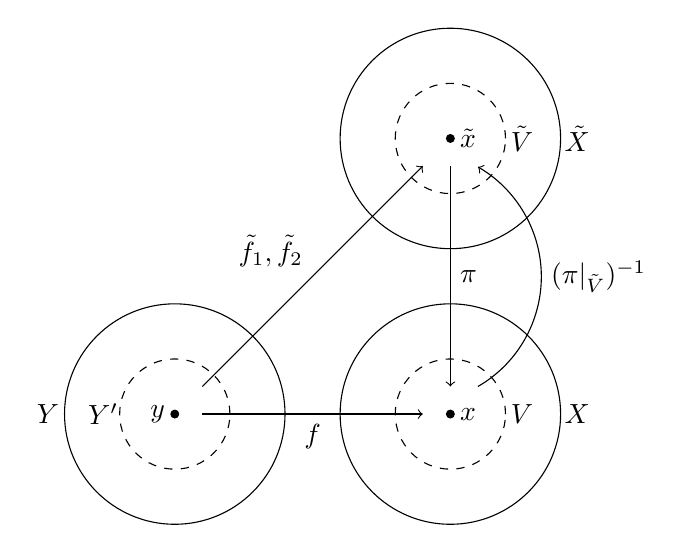
\begin{tikzpicture}[scale=0.7]
  % Draw the space X and its neighborhood V
  \draw (0,0) circle (2cm); % Space X
  \node at (2.3,0) {\(X\)};
  \draw[dashed] (0,0) circle (1cm); % Neighborhood V
  \node at (1.3,0) {\(V\)};
  \filldraw[black] (0, 0) circle (2pt) node[right] {$x$}; % Point x

  % Draw the covering space \tilde{X} and its neighborhood \tilde{V}
  \draw (0,5) circle (2cm); % Space tilde X
  \node at (2.3,5) {\(\tilde{X}\)};
  \draw[dashed] (0,5) circle (1cm); % Neighborhood tilde V
  \node at (1.3,5) {\(\tilde{V}\)};
  \filldraw[black] (0, 5) circle (2pt) node[right] {$\tilde{x}$}; % Point tilde x

  % % Draw the space Y and its neighborhood Y'
  \draw (-5,0) circle (2cm);
  \node at (-2.3-5,0) {\(Y\)};
  \draw[dashed] (-5,0) circle (1cm); 
  \node at (-1.3-5,0) {\(Y'\)};
  \filldraw[black] (-5, 0) circle (2pt) node[left] {$y$}; 

  % % Arrows representing maps
  \draw[->] (-5+0.5,0) -- (-0.5,0) node[midway, below] {\(f\)}; % f: Y -> X
  \draw[->] (-5+0.5,0.5) -- (0-0.5,5-0.5) node[midway, above left] {\(\tilde{f}_1, \tilde{f}_2\)}; % \tilde{f}_1, \tilde{f}_2: Y -> \tilde{X}
  \draw[->] (0,4.5) -- (0,0.5) node[midway, right] {\(\pi\)}; % \pi: \tilde{X} -> X
  \draw[->] (0.5,0.5) arc[start angle=-60, end angle=60, radius=2.3] node[midway, right] {\((\pi|_{\tilde{V}})^{-1}\)};
\end{tikzpicture}
\end{center}
\end{proof}

Since we have proven a uniqueness result, it is natural to wonder about an existence result.
It is not the case that it is always possible to lift a given map.
So instead, in the following theorem we examine how a lift changes as the base map changes. 
We conceive of $f : Y \to X$ as depending on a ``time'' parameter $t$.
More properly, we have a map $F : Y \times [0,1] \to X$.
We prove that if a lift exists at time $t=0$ then it also exists for any time $t \in [0,1]$.

\begin{theorem}[Homotopy Lifting Property]
\label{thm:homotopy lifting property}
\textup{\cite[Thm~3.23]{Warner1983}\cite[Thm~1.7(c)]{Hatcher2002}}\\
Let $\pi : \tilde{X} \to X$ be a covering map.
Given a map $F : Y \times [0,1] \to X$ and a map $\tilde{F}_0 : Y \times \{0\} \to \tilde{X}$ lifting $F|_{Y \times \{0\}}$ there is a unique map $\tilde{F} : Y \times [0,1] \to \tilde{X}$ lifting $F$ such that $\tilde{F}|_{Y \times \{0\}} = \tilde{F}_0$.
\[
\begin{tikzcd}[sep=large]
Y \times \{0\} \arrow[r, "\tilde{F}_0"] \arrow[d, hook] & \tilde{X} \arrow[d, "\pi"] \\
Y \times [0,1] \arrow[r, "F"] \arrow[ru, "\tilde{F}"] & X
\end{tikzcd}
\]
\end{theorem}
\begin{proof}
First we set up a special cover on $Y\times[0,1]$.
For any point $(y,s) \in Y \times [0,1]$ its image $F(y,s)$ is contained in an evenly covered subset $V$ of $X$.
In $F^{-1}[V]$ we can find an open rectangle $N' \times (a,b)$ containing $(y,s)$.
Applying this for every point, we get a cover $\{ N'_i \times (a_i,b_i) \}$ of $Y \times [0,1]$.
But we are not yet done.
For any $y \in Y$, consider the subcover $\{ N'_i \times (a_i,b_i) | y \in N'_i \}$.
This covers $\{y\}\times [0,1]$.
As it is a compact space there is a finite subcover; let it be indexed by $\mathcal{K}_y$.
Then define $N_y$ to be the connected component of $\bigcap_{k \in \mathcal{K}_y} N'_k \subset Y$ that contains $y$.
It is open, because the intersection of open sets is finite.
This cover $\{N_y \times (a_k,b_k)\}_{y \in Y, k \in \mathcal{K}_y}$ is the special cover of $Y \times [0,1]$ that we wanted to construct.
It has the property that for each $y$ there is the finite subcover $\{N_y \times I_k\}_{k \in \mathcal{K}_y}$ of $N_y\times [0,1] \supset \{y\} \times [0,1]$.
\begin{center}
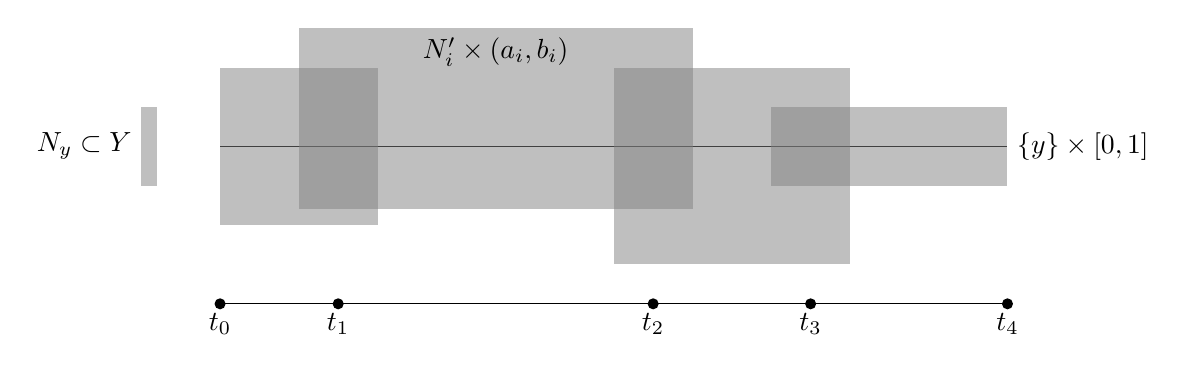
\begin{tikzpicture}
% Draw the horizontal line
\draw (0,0) -- (10,0) node[right]{$\{y\} \times [0,1]$};

% Draw the overlapping rectangles
\fill[gray, opacity=0.5] (0,-1) rectangle (2,1);
\fill[gray, opacity=0.5] (1,-0.8) rectangle (6,1.5);
\draw (3.5,1.5) node[below]{$N'_i\times(a_i,b_i)$};
\fill[gray, opacity=0.5] (5,-1.5) rectangle (8,1);
\fill[gray, opacity=0.5] (7,-0.5) rectangle (10,0.5);

% Draw the intersection N
\fill[gray, opacity=0.5] (-1,-0.5) rectangle (-0.8,0.5);
\draw (-1,0) node[left]{$N_y \subset Y$};

% Draw the partition
\draw (0,-2) -- (10,-2);
\fill (0, -2) circle (2pt) node[below]{$t_0$};
\fill (1.5, -2) circle (2pt) node[below]{$t_1$};
\fill (5.5, -2) circle (2pt) node[below]{$t_2$};
\fill (7.5, -2) circle (2pt) node[below]{$t_3$};
\fill (10, -2) circle (2pt) node[below]{$t_4$};
\end{tikzpicture}
\end{center}

In the next step, we construct ``local lifts''.
That means for any point $y \in Y$ construct a lift of $F$ restricted to $N_y\times[0,1]$.
The argument is constructive but inductive.
Fix $y \in Y$ and choose a partition $0 = t_0 < t_1 < \dots < t_n = 1$ of $[0,1]$ so that each $[t_j, t_{j+1}]$ belongs to an interval $(a_k,b_k)$ for some $k \in \mathcal{K}_{y}$.
By the construction of the cover, $F[N_{y} \times [t_j,t_{j+1}]] \subset F[N_y \times (a_k,b_k)]$ is contained in an evenly covered set $V_j \subset X$.

Assume inductively that we have constructed the lift $\tilde{F}$ on $N_y \times [0,t_j]$.
This means $\pi(\tilde{F}(y',t_j)) = F(y',t_j)$, or in other words $\tilde{F}(y',t_j) \in \pi^{-1}[F(y',t_j)]$ for all $y' \in N_{y}$.
Let $\tilde{V}_j \subset \tilde{X}$ be the sheet of $V_j$ that contains $\tilde{F}(y,t_j)$.
Then in fact it contains all of $\tilde{F}[N_{y}\times\{t_j\}]$ since this set is connected.
Now we extend the definition of $\tilde{F}$ by using the local inverse $\pi^{-1} : V_j \to \tilde{V}_j$:
\[
\tilde{F}(y', t') = \pi^{-1} \circ F(y',t') \text{ for } y' \in N_y,\; t' \in [t_j,t_{j+1}].
\]

The base case of the induction $j=0$ is trivial: we need to construct a lift of $F$ on $N_y\times[0,0]$, but we already have $\tilde{F}_0$ given to us in the theorem.
This finishes the proof of the existence of local lifts.

Finally, we use local existence and uniqueness to patch these together into a global function.
Indeed, suppose that $\tilde{F}_y$ is the local lift on $V_{y}\times[0,1]$.
If there is a point $y \in V_{y_1}\cap V_{y_2}$ we know that $\Tilde{F}_{y_1}(y,0) = \Tilde{F}_0(y) = \Tilde{F}_{y_2}(y,0)$, and hence by uniqueness of lifts they agree everywhere on $(V_{y_1}\cap V_{y_2})\times[0,1]$.
So we may safely define $\tilde{F}(y,t) = \tilde{F}_y(y,t)$.
\end{proof}

Note that $\tilde{F}$ is defined essentially as the composite of $\pi^{-1}$ and $F$ on suitable patches.
In particular, this shows us its regularity.
For instance, if $\pi$ and $F$ are smooth then so is $\tilde{F}$.

There are two special cases of this theorem that are used more than any others.
The first is the case that $Y$ is a one point space, in which case it plays no role.
Then we can interpret $F$ as a path $[0,1] \to X$.
The initial lift $\tilde{F}_0$ is nothing other than a choice of point in $\pi^{-1}[F(0)]$.
Thus every curve has a lift, unique up to choice of starting point in $\tilde{X}$ lying over the starting point in $X$.

The second use is when $F$ is the homotopy of two curves relative their endpoints.
Let us define the concept of homotopy.
\begin{definition}
\label{def:homotopy}
Given two functions $f,g : Y \to X$ a homotopy relative $K \subset Y$ is a function $F : Y \times [0,1] \to X$ such that $F(y,0) = f(y)$ and $F(y,1) = g(y)$ for all $y \in Y$, and $F(k,t) = f(k) = g(k)$ for all $k\in K, t\in[0,1]$.
We say that the maps are homotopic relative $K$.
\end{definition}
In the case of curves we use $Y = [a,b]$ and $K = \{a,b\}$.
A map $f : [a,b] \to X$ is a path into $X$.
If $f$ is homotopic to $g$ relative $K$ then there is deformation of $f$ into $g$ such that the endpoints of the curves are not moved.
From the previous paragraph, both of the curves can be lifted with the same starting points.
The fact that the homotopy can be lifted tells us that the two curves are homotopic in the covering space.
In particular, they have the same finishing points $\tilde{f}(b) = \tilde{g}(b)$. 

Since we have defined homotopy, let us also define the fundamental group of a space.
\begin{definition}
\label{def:fundamental group}
Fix a point $x_0 \in X$ and consider loops based at $x_0$: continuous paths $\gamma : [0,1] \to X$ with $\gamma(0) = \gamma(1) = x_0$.
We consider the set $\pi_1(X,x_0)$, called the fundamental group of $X$, of loops up to homotopy relative $x_0$.
\end{definition}
We can equip this with an operation, namely concatenation of loops
\[
(\beta \cdot \alpha)(s)
= \begin{cases}
\alpha(2s) & \text{if } s\leq 0.5 \\
\beta(2s-1) & \text{if } s> 0.5
\end{cases}.
\]
The identity is the constant path at $x_0$ and inverse is traversal of the loop in the opposite direction
\[
\gamma^{-1}(s) = \gamma(1-s).
\]
Properly, we should prove these claims.
As an example of verifying that this does in fact make $\pi_1(X,x_0)$ a group, 
\[
F(s,t) = \begin{cases}
\gamma(2st) & \text{if } s\leq 0.5 \\
\gamma(2(1-s)t) & \text{if } s> 0.5
\end{cases}
\]
is a homotopy between the identity loop $F(s,0) = \gamma(0) = x_0$ and $F(s,1) = \gamma^{-1} \cdot \gamma$.
We leave the remaining checks to the reader.

These ideas together give the existence of a lift of any map from a simply connected space.
A simply connected space is a connected space in which every loop is homotopic to a constant map.
Equivalently, the fundamental group is the trivial group with one element.
Be aware, not every author requires simply connected spaces to be connected (and not every author is consistent).
\begin{corollary}[Lifting existence]
\textup{\cite[Prop~1.33]{Hatcher2002}}
\label{cor:lift existence}
Let $\pi : \tilde{X} \to X$ be a covering.
Suppose that $Y$ is simply connected.
This means that any two paths in $Y$ with the same endpoints are homotopic.
Then given a map $f : Y \to X$ and points $y \in Y$ and $\tilde{x} \in \pi^{-1}[f(y)]$, there exists a unique lift $\tilde{f}$ of $f$ with $\tilde{f}(y) = \tilde{x}$.
\[\begin{tikzcd}[sep=large]
& (\tilde{X},\tilde{x}) \arrow{d}{\pi} \\
(Y,y) \arrow{r}{f} \arrow[dashed]{ru}{\tilde{f}} & (X,x)
\end{tikzcd}\]
\end{corollary}
\begin{proof}
For any point $y' \in Y$, let $\gamma : [0,1] \to Y$ be a path between $y$ and $y'$.
Then by the discussion above, the path $f \circ \gamma$ has a lift $\tilde{\gamma} : [0,1] \to \tilde{X}$ with $\tilde{\gamma}(0) = \tilde{x}$.
Define $\tilde{f}(y') = \tilde{\gamma}(1)$.
This is well-defined, because if there is any other path $\gamma_2$ to $y'$, then by assumption there is a homotopy $F$ between the two paths.
Then $f\circ F$ is a homotopy of $f\circ\gamma$ and $f\circ\gamma_2$.
But we know, again from the discussion above, that the lifts of homotopic paths have the same finishing point $\tilde{f}(y') = \tilde{\gamma}(1) = \tilde{\gamma}_2(1)$.
\end{proof}

Simply connected spaces play a special role in the theory of covering spaces.
If $\pi : \tilde{X} \to X$ is a covering map and $\tilde{X}$ is simply connected (and connected), we say that $\tilde{X}$ is a \emph{universal cover} of $X$.
The reason for the epitaph `universal' is that if $\pi : Y \to X$ is any covering map, and $\pi_X : \tilde{X} \to X$ is a universal cover, then the lifting property tells us that $\pi_X$ lifts to a map $\pi_Y$ to $Y$, with $\pi_X = \pi \circ \pi_Y$.
\[\begin{tikzcd}[sep=large]
\tilde{X} \arrow{rd}{\pi_X} \arrow[dashed]{rr}{\pi_Y} && Y \arrow{ld}{\pi} \\
& X &
\end{tikzcd}\]
If $Y$ is connected, then we claim that this lift is itself a covering map.
For any point of $X$ take a neighborhood that is evenly covered by both $\pi_X$ and $\pi$.
If $U_y \subset Y$ and $V_{\tilde{x}} \subset \tilde{X}$ are sheets, then
\[
(\pi|_{U_y})^{-1} \circ \pi_X : \coprod_{\tilde{x} \in \pi_Y^{-1}[y]} V_{\tilde{x}} \to U_y
\]
is an even covering of the neighborhood $U_y$ of $y$.
This shows that $\pi_Y$ is a local diffeomorphism, and in particular both open and closed.
Since $Y$ is connected, the image of $\tilde{X}$ in $Y$ must be the whole space.
This shows that $\pi_Y$ is surjective.
Therefore $\pi_Y$ is a covering.
A universal cover is in this sense the largest connected space that covers $X$.
We often speak of the universal cover, because if there are two simply connected covering spaces, we can apply this reasoning to construct a diffeomorphism between them.

\begin{corollary}
The universal cover is unique in the following sense:
If $\tilde{X},\tilde{X}'$ are simply connected and $\pi : \tilde{X} \to X, \pi': \tilde{X}'\to X$ are covering maps, then for any points $x \in X$, $\tilde{x} \in \pi^{-1}[x]$, and $\tilde{x}' \in \pi^{-1}[x]$ there is a diffeomorphism from $\tilde{X}$ to $\tilde{X}'$ that takes $\tilde{x}$ to $\tilde{x}'$.
\qed
\end{corollary}

% DECK TRANSFORMATIONS:
% We can apply this corollary to the universal cover itself.
% Given two points $\tilde{x},\tilde{x}' \in \pi^{-1}[x]$ there is an automorphism of $\tilde{X}$ taking $\tilde{x}$ to $\tilde{x}'$.
% These automorphisms are called deck transformations of $\pi$.
% The set of deck transformations of the universal cover acts transitively on the fibre of any point.



\section{Eigenvalues and Weights}

Eigenvalues and eigenvectors are ubiquitous in linear algebra.
If we are working over $\bbC$, then every linear endomorphism (linear map from a vector space $V$ to itself) has an eigenvalue (root of the characteristic polynomial) and every eigenvalue has an eigenvector $Av_\lambda = \lambda v_\lambda$.
If we can find a basis of eigenvectors, then with respect to this basis the linear operator is a diagonal matrix.
In general however, there may be fewer eigenvectors than the dimension of the vector space.
A standard result in linear algebra says that every matrix is conjugate to a matrix in Jordan normal form, unique up to reordering of the blocks.

Going further, we may ask what can be said of two linear endomorphisms $A,B$.
The key observation is to consider commuting operators.
If $A$ and $B$ commute then $B$ preserves the eigenspaces of $A$:
\[
(A- \lambda I) (Bv) 
= B(A- \lambda I) v
= 0.
\]
Therefore $B$ restricts to an endomorphism on each of the eigenspaces of $A$.
Imposing different conditions on $A$ restricts the possible decompositions of $B$.
For example, if $A$ is diagonalizable (so $V$ decomposes as the direct sum of the eigenspaces of $A$) then on each eigenspace of $A$ we can choose a basis that puts $B$ into Jordan normal form.
Hence $A$ and $B$ can be simultaneously conjugated to normal form.
Or if $A$ is diagonalizable and has no repeated eigenvalues, ie its eigenspaces are one dimensional, then these must also be eigenspaces of $B$.
Hence $A$ and $B$ are simultaneously diagonalizable.

This argument can be applied inductively to a finite set $\{A_1,\dots,A_k\}$ of pairwise commuting endomorphisms.
It also extends to a commuting family of operators $\mathcal{A} = \vspan\{A_1,\dots,A_k\}$, a linear subspace of $\End(V)$ such that all operators are pairwise commuting.
These are effectively equivalent, since a family is pairwise commuting if and only if a basis is pairwise commuting.
Likewise, $v$ is a simultaneous eigenvector for $\{A_1,\dots,A_k\}$ if and only if it is a simultaneous eigenvector for every operator of $\mathcal{A}$.
The eigenvalues are not completely independent:
\[
\lambda v
= Av 
= (a_1A_1 + \dots + a_kA_k)v
= a_1 \lambda_1 v + \dots + a_k \lambda_k v
= (a_1 \lambda_1 + \dots + a_k \lambda_k )v.
\]
We understand the eigenvalue of $v$ to be a linear function 
\[
\lambda : \mathcal{A} \to \mathbb{K}, 
\quad
\lambda(A) = a_1 \lambda_1 + \dots + a_k \lambda_k .
\]
Understood in this way, it is more common to call $\lambda$ a \emph{weight} of the commuting family $\mathcal{A}$, $v$ a \emph{weight vector}, and the set of vectors $v$ with $Av = \lambda(A)v$ the \emph{weight} space~\cite[Definition~A.14]{Hall2015}.

As an aside, the descriptor ``weight'' should probably replace ``eigen-'' even in the single operator case.
Consider an operator $A$ with a $2$-weight vector $v$ and a $3$-weight vector $w$.
Then of course $A(v+w) = 2v + 3w$, which is a weighted sum.

We finish with an example.
Let $\mathcal{A}$ be the set of diagonal $n\times n$ matrices.
Then a basis for this family is $A_i = e_{ii}$, with $1$ at the $i$th position on the diagonal.
$e_i$ is a $1$-weight vector of $A_i$ while all vectors of $\vspan\{e_1,\dots,\hat{e}_i,\dots,e_n\}$ are $0$-weight (in the kernel).
These are all diagonal (in particular simultaneously diagonal) so there should be a basis of weight vectors.
Indeed, this is just the standard basis $\{e_1,\dots,e_n\}$.
The weight of $e_i$ is the linear form
\[
A = \operatorname{diag}(a_1,\dots,a_n) \mapsto a_i
\]
because $A e_i = a_i$.

